\documentclass{article}
\usepackage[margin=1in]{geometry}
\usepackage{amsmath}
\usepackage{graphicx}
\usepackage{hyperref}
\usepackage{float} % Used for the [H] figure placement option

\title{Solving a Stochastic Gridworld Problem using Q-Learning}
\author{Varun Karthik, Jeevan Hebbal Manujanath, Yeshwanth Reddy Gurureddy}
\date{\today}

\begin{document}

\maketitle
\tableofcontents % Adds a table of contents
\newpage

\begin{abstract}
This report details the application of the Q-learning algorithm to solve a stochastic 3x4 Gridworld problem. The objective is to find an optimal policy that maximizes the cumulative reward. We explore the fundamental concepts of Q-learning, analyze the impact of key hyperparameters on the agent's performance, and discuss the convergence properties of the Q-values versus the learned policy. The analysis is supported by empirical results generated from a Python implementation of the Q-learning agent.
\end{abstract}

\section{Introduction to Q-Learning}

Reinforcement Learning (RL) is a paradigm of machine learning where an agent learns to make decisions by interacting with an environment. The agent performs actions, receives rewards (or penalties), and observes new states, learning a policy that maximizes its long-term reward.

Q-learning is a model-free, off-policy RL algorithm. "Model-free" means it does not need a model of the environment's dynamics (i.e., it doesn't need to know the transition probabilities). It learns the value of actions directly from experience. Its primary goal is to learn an action-value function, denoted as $Q(s, a)$, which represents the expected cumulative discounted reward of taking action $a$ in state $s$ and following the optimal policy thereafter.

\subsection{The Gridworld Environment}
The problem is set in a 3x4 grid. The agent's goal is to navigate from a `START` state at (1,1) to one of two terminal states: a goal state at (4,3) with a reward of $+1$ and a penalty state at (4,2) with a reward of $-1$. All other movements incur a small negative reward of $-0.04$ to encourage efficiency. The environment is stochastic: an intended action is successful only 80\% of the time. There is a 10\% chance of moving to the left of the intended direction and a 10\% chance of moving to the right.

\section{Methodology}

\subsection{The Q-Function and Update Rule}
The core of the algorithm is the iterative updating of the Q-function based on the agent's experiences. This update is derived from the Bellman equation and is performed using the following rule:
$$
Q(s_t, a_t) \leftarrow Q(s_t, a_t) + \alpha \left[ R_{t+1} + \gamma \max_{a} Q(s_{t+1}, a) - Q(s_t, a_t) \right]
$$
Where:
\begin{itemize}
    \item $s_t$ and $a_t$ are the current state and action.
    \item $R_{t+1}$ is the reward received after performing action $a_t$.
    \item $s_{t+1}$ is the next state.
    \item $\alpha$ is the \textbf{learning rate}, controlling how much new information overrides old information.
    \item $\gamma$ is the \textbf{discount factor}, determining the importance of future rewards.
    \item $\max_{a} Q(s_{t+1}, a)$ is the agent's estimate of the best possible future value from state $s_{t+1}$.
\end{itemize}

\subsection{Exploration vs. Exploitation}
To discover the optimal policy, the agent must balance exploring new actions with exploiting actions that have proven to be effective. We use an $\epsilon$-greedy strategy:
\begin{itemize}
    \item With probability $\epsilon$, the agent chooses a random action (exploration).
    \item With probability $1-\epsilon$, the agent chooses the action with the highest Q-value for the current state (exploitation).
\end{itemize}
To ensure convergence, $\epsilon$ is gradually decayed over time, shifting the agent's focus from exploration to exploitation as it learns more about the environment.

\section{Results and Discussion}
The agent was trained for 20,000 episodes, and its performance was evaluated based on the effect of different hyperparameters.

\subsection{Effect of Hyperparameters}
The choice of hyperparameters significantly affects the agent's learning efficiency and final performance.

\subsubsection{Learning Rate ($\alpha$)}
As shown in Figure~\ref{fig:learning_rate}, the learning rate dictates how quickly the agent adapts. A low $\alpha$ (0.01) leads to slow but stable learning, while a high $\alpha$ (0.9) causes instability. An optimal value of $\alpha=0.1$ provides a balance, allowing for rapid yet stable convergence.

\begin{figure}[H]
    \centering
    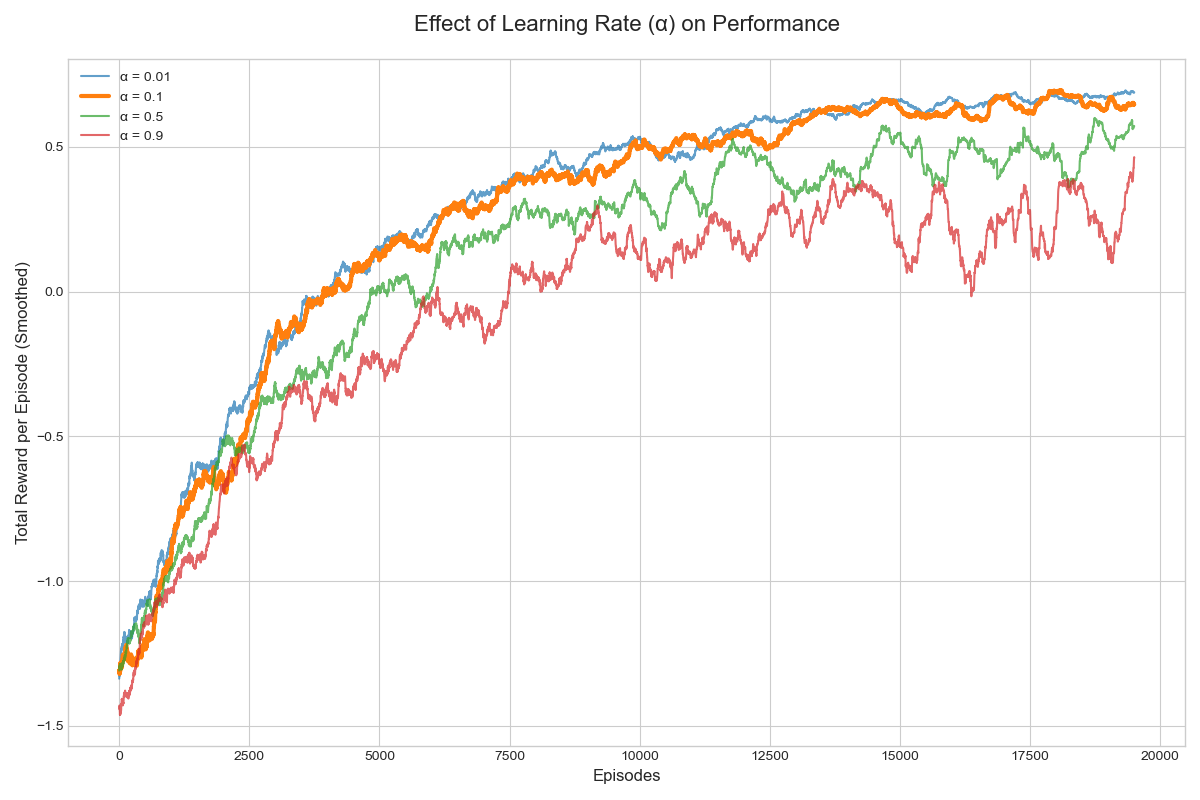
\includegraphics[width=0.6\textwidth]{../results/learning_rate_vs_episodes.png}
    \caption{Effect of Learning Rate ($\alpha$) on Performance. The optimal value of 0.1 shows a smooth and rapid convergence to a high reward.}
    \label{fig:learning_rate}
\end{figure}

\subsubsection{Discount Factor ($\gamma$)}
The discount factor controls the agent's foresight. Figure~\ref{fig:discount_factor} shows that a higher $\gamma$ (e.g., 0.99) is essential for the agent to value the distant +1 reward and find the optimal path. Lower values make the agent too "short-sighted."

\begin{figure}[H]
    \centering
    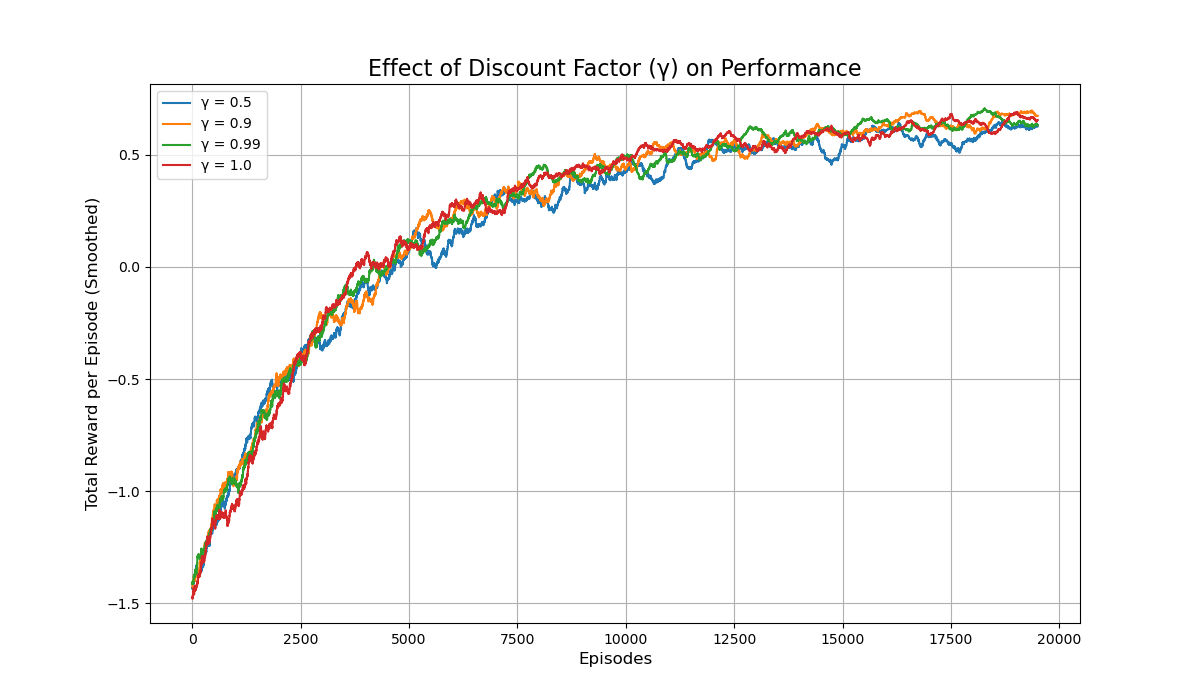
\includegraphics[width=0.6\textwidth]{../results/discount_factor_episodes.png}
    \caption{Effect of Discount Factor ($\gamma$) on Performance. Higher values that encourage looking far into the future lead to better overall rewards.}
    \label{fig:discount_factor}
\end{figure}


\subsubsection{Epsilon ($\epsilon$) Decay Schedule}
The rate at which the agent reduces exploration is crucial. Figure~\ref{fig:epsilon_decay} illustrates this trade-off. A fast decay (0.999) causes the agent to stop exploring too early, settling on a suboptimal policy. A slow decay (0.99999) wastes too much time on random actions. The optimal rate (0.9999) allows for sufficient exploration before committing to the best-found policy.

\begin{figure}[H]
    \centering
    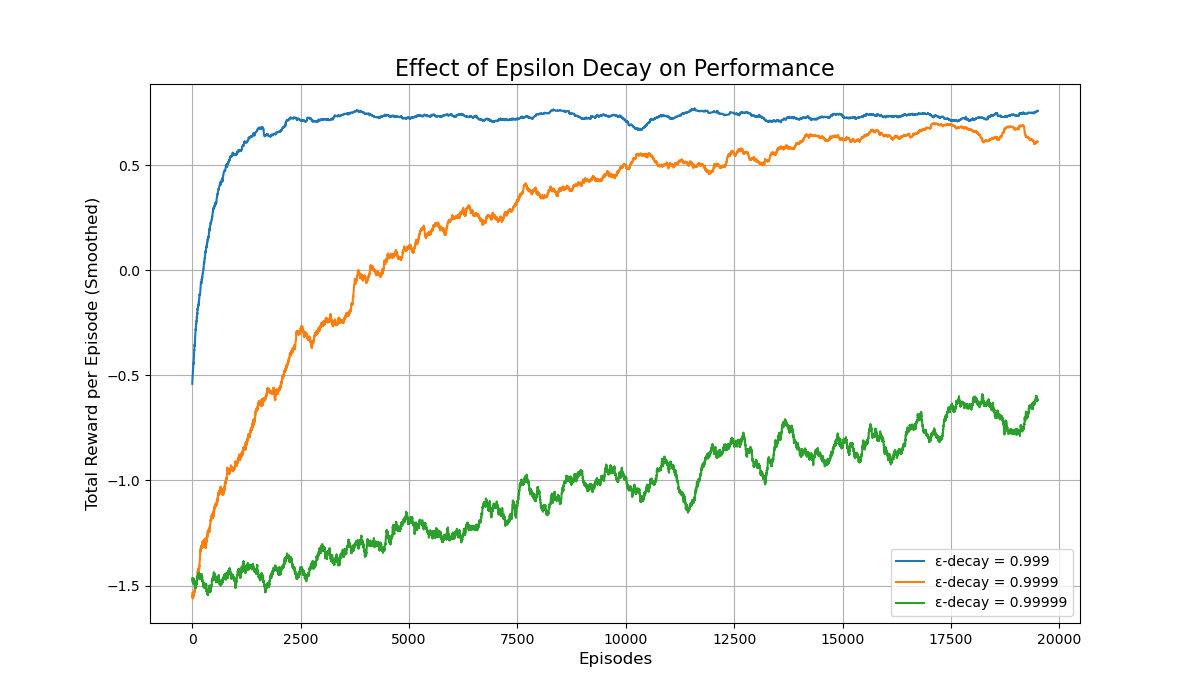
\includegraphics[width=0.6\textwidth]{../results/epsilon_decay.png}
    \caption{Effect of Epsilon ($\epsilon$) Decay on Performance. A balanced decay rate is critical for effective learning.}
    \label{fig:epsilon_decay}
\end{figure}

\subsection{Convergence of Q-Values vs. Policy}
The results strongly indicate that \textbf{the policy converges before the Q-values}. An agent's policy is determined by the \textit{relative} ranking of Q-values for actions in a given state ($\arg\max_a Q(s, a)$). This ranking can stabilize long before the Q-values themselves stop changing.

Figure~\ref{fig:policy_heatmap} shows the clear, stable final policy. In contrast, Figure~\ref{fig:q_convergence} shows that the specific Q-value for taking 'Up' in the start state is still being refined late into training, even though the policy itself has likely been fixed for thousands of episodes.

\begin{figure}[H]
    \centering
    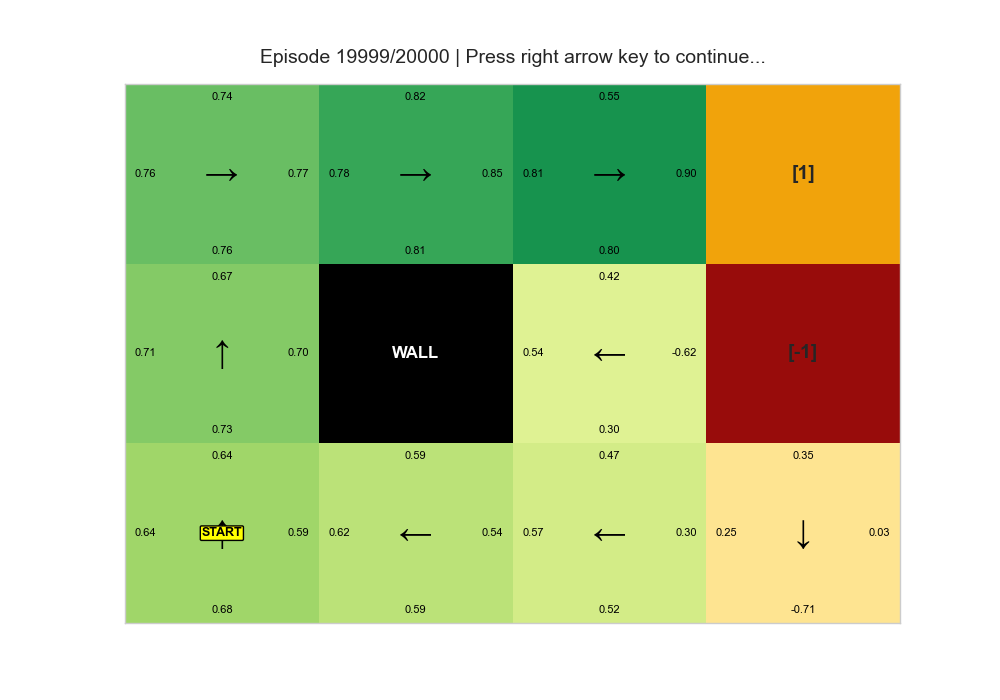
\includegraphics[width=0.6\textwidth]{../results/qpolicy_visualizatoin_heatmapt.png}
    \caption{The final learned policy and Q-value heatmap after 20,000 episodes. The arrows indicate a clear, optimal path to the +1 reward.}
    \label{fig:policy_heatmap}
\end{figure}

\begin{figure}[H]
    \centering
    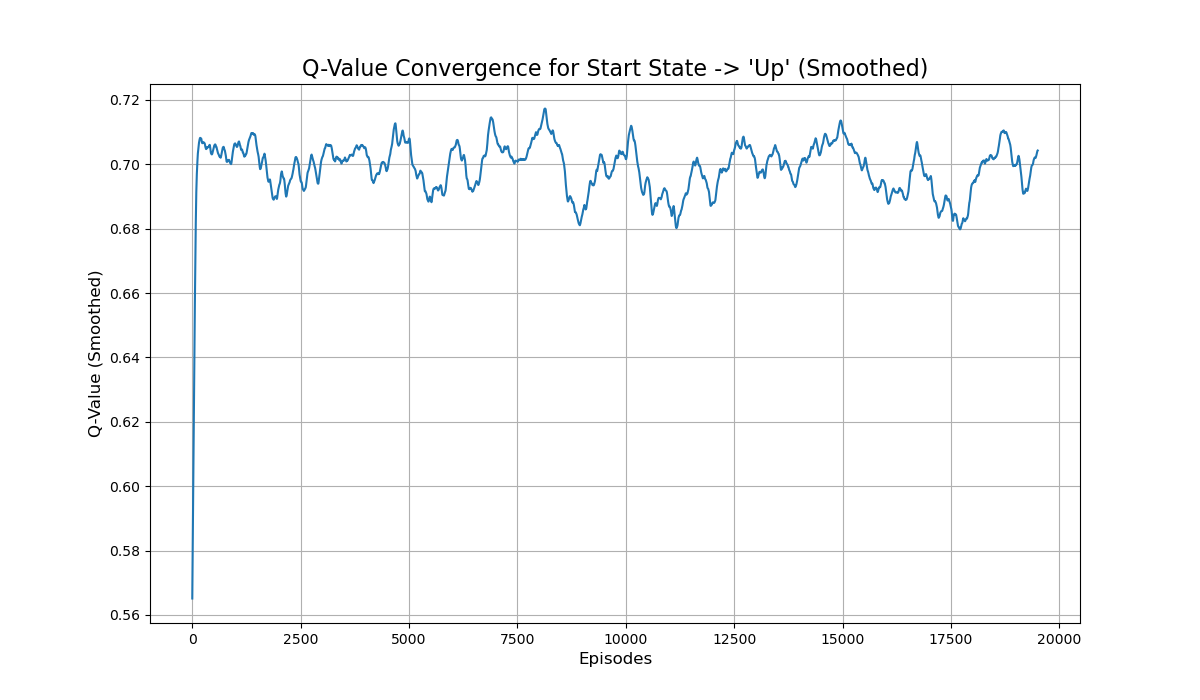
\includegraphics[width=0.6\textwidth]{../results/qvalue_vs_episodes.png}
    \caption{Convergence of a single Q-value (Start State, Action 'Up'). The value continues to fluctuate and be refined even after the policy has stabilized.}
    \label{fig:q_convergence}
\end{figure}

\subsection{Effect of Increased Penalty}
When the penalty at state (4,2) was increased from -1 to -200, the agent learned a much more conservative policy. It learns to take a longer route that gives the penalty state a wide berth, ensuring that even with the 10\% probability of deviation, it avoids the massive penalty. This demonstrates the algorithm's ability to adapt its policy to reflect the magnitude of risks and rewards in the environment.

\section{Conclusion}
Q-learning successfully determined an optimal policy for the stochastic Gridworld. The analysis demonstrates the critical role of hyperparameter tuning in achieving efficient learning. We observed that an agent's policy converges substantially earlier than its underlying Q-values. The model's adaptation to a drastically increased penalty highlights its robustness and ability to learn risk-averse behavior.

\end{document}
